% LaTeX-Vorlage Version 3.1,  Juli 2011
% erstellt von Dr. Andreas Drauschke (andreas.drauschke@technikum-wien.at) und Dr. Susanne Teschl (susanne.teschl@technikum-wien.at)
% geringf"ugig adaptiert von Harald Stockinger (harald.stockinger@technikum-wien.at)

 
\documentclass[a4paper,bibtotoc,oneside]{scrbook} 
% F"ur kurze Arbeiten w"are auch die Dokumentklasse "scrartcl" ausreichend. In diesem Fall ist "section" die h"ochste Ebene ("chapter" gibt es dann nicht).
% \documentclass[a4paper,bibtotoc,oneside]{scrartcl}


% verlinkte Querverweise im pdf
\usepackage{hyperref}

% deutsche Anpassungen
%\usepackage[ansinew]{inputenc}
\usepackage[utf8]{inputenc}
\usepackage[T1]{fontenc}
\usepackage[ngerman]{babel}




% mathematische Symbole
\usepackage{amsmath,amssymb,amsfonts,amstext}

% Kopfzeilen frei gestaltbar
\usepackage{fancyhdr}
\lfoot[\fancyplain{}{}]{\fancyplain{}{}}
\rfoot[\fancyplain{}{}]{\fancyplain{}{}}
\cfoot[\fancyplain{}{\footnotesize\thepage}]{\fancyplain{}{\footnotesize\thepage}}
\lhead[\fancyplain{}{\footnotesize\nouppercase\leftmark}]{\fancyplain{}{}}
\chead{}
\rhead[\fancyplain{}{}]{\fancyplain{}{\footnotesize\nouppercase\sc\leftmark}} 

% Farben im Dokument m"oglich
\usepackage{color}

% Schriftart Helvetica
\usepackage{helvet}
\renewcommand{\familydefault}{cmss} 

% Graphiken einbinden: hier f"ur pdflatex
\usepackage[pdftex]{graphicx}

\usepackage{array}

% H"ohe und Breite des Textk"orpers etwas gr"osser definieren
\setlength{\textheight}{225mm}
\setlength{\textwidth}{1.05\textwidth}

% weniger Warnungen wegen "uberf"ullter Boxen
\tolerance = 9999
\sloppy

% Anpassung einiger "Uberschriften 
\renewcommand\figurename{Abbildung}
\renewcommand\tablename{Tabelle}



\begin{document}

% Kopf- und Fusszeilen initiieren
\pagestyle{fancy}

% Deckblatt:
\thispagestyle{empty}
\begin{picture}(0,0)
\color{white}\sffamily
\put(-101,-749){
\includegraphics[width=1.002\paperwidth, height=\paperheight]{img/BM_2011.pdf}}
\put(220,-670){
\includegraphics[width=0.5\textwidth]{img/FHTW_Logo_4c.pdf}}
\put(-30, -20){\bfseries\huge MASTER THESIS}
\put(-30,-50){\Large zur Erlangung des akademischen Grades}
\put(-30,-70){\Large \glqq Master of Science in Engineering\grqq}
% Titel des Studienganges einf"ugen:
\put(-30,-90){\Large im Studiengang Industrielle Elektronik}
% Titel der Arbeit einf"ugen:
% Die Minipage wird gesetzt, damit auch mehrzeilige Titel m"oglich werden.
\put(-32,-180){
\begin{minipage}{14cm}
\bfseries\huge Aufbau eines automatisierten Mess- und Auswertesystems zur Bestimmung der Bestrahlungsst"arkeverteilung in einem station"aren Sonnensimulator
\end{minipage}
}
% Name der Autorin/des Autors eingeben:
\put(-30,-270){\large Ausgef"uhrt von: Thomas Schmatz BSc}
% Personenkennzeichen der Autorin/des Autors eingeben:
\put(-30,-290){\large Personenkennzeichen: 1010300002}
% Name der Begutachterinnen/der Begutachter eingeben:
\put(-30,-330){\large 1. BegutachterIn: DI Bernhard Kubicek}
\put(-30,-350){\large 2. BegutachterIn: DI (FH) Thomas Krametz }
\put(-30,-390){\large Wien, \today} % das Datum des letzten Kompilierens wird automatisch eingesetzt
\color{black}
\end{picture}

\newpage


\section*{Eidesstattliche Erkl"arung}\thispagestyle{empty}
\glqq Ich erkl"are hiermit an Eides statt, dass ich die vorliegende Arbeit selbst"andig angefertigt habe. 
Die aus fremden Quellen direkt oder indirekt "ubernommenen Gedanken sind als solche kenntlich gemacht. 
Die Arbeit wurde bisher weder in gleicher noch in "ahnlicher Form einer anderen Pr"ufungsbeh"orde vorgelegt
und auch noch nicht ver"offentlicht. Ich versichere, dass die abgegebene Version jener im Uploadtool entspricht.\grqq\\[5\baselineskip]
\rule{5cm}{0.2pt}\hfill\rule{5cm}{0.2pt}\\
\phantom{Datum }Ort, Datum\hfill Unterschrift\hspace{15mm}

\newpage



\section*{Kurzfassung}\thispagestyle{empty}
Die Arbeit umfasst die Planung und Realisierung eines selbstfahrenden Messroboters, der die Bestrahlungsst"arkeverteilung in der Prüfebene eines station"aren Sonnensimulators erfasst. Neben den Einstrahlungsdaten werden werden zus"atzliche Informationen über die Umgebungsbedingungen im Prüfkanal aufgezeichnet. Bei der Umsetzung wurden Rapid-Prototyping Techniken (3D-Druck, Platinenfr"ase und Lasercutter) eingesetzt. Behandelt werden theoretische Grundlagen und normative Anforderungen an station"are Sonnensimulatoren, sowie Messunsicherheitsberechnungen und Validierung des Gesamtsystems.
\\ \vfill
% Bitte 3-5 deutsche Schlagw"orter eingeben, die die Arbeit charakterisieren:
\paragraph*{Schlagw"orter:} Schlagwort 1, Schlagwort 2, Schlagwort 3, Schlagwort 4, Schlagwort 5


\newpage

\section*{Abstract}\thispagestyle{empty}
Text Text Text Text Text Text Text Text Text Text Text Text Text Text Text Text Text Text Text Text Text Text Text Text ...
\\ \vfill
% Bitte 3-5 englische Keywords eingeben, die die Arbeit charakterisieren:
\paragraph*{Keywords:} Keyword 1, Keyword 2, Keyword 3, Keyword 4, Keyword 5
\newpage

\section*{Danksagung}\thispagestyle{empty}
Ich danke meinen Eltern für die Unterstützung und Geduld, die sie w"ahrend des Studiums aufgebracht haben.
Ich danke meinen Hochschulbetreuer für die umfangreiche Betreuung.
Ich danke meinen Firmenbetreuer Thomas Krametz für die Zeit die er sich genommen hat.
... (Rohfassung!!!!)
\newpage

\tableofcontents\thispagestyle{empty}
\newpage

\setcounter{page}{1}

% Falls die Kapitel"uberschriften zu lang f"ur die Kopfzeile oder das Inhaltsverzeichnis sind, so erzielt man
% dort Kurzformen der Kapitelbezeichnungen mittels:
% \chapter[Kurzform]{Lange "Uberschrift}
\chapter{Aufgabenstellung}
\section{Warum Module im Sonnensimulator} 
Ein Sonnensimulator simuliert die Wirkung von Sonnenlicht auf Pr"ufobjekte.

\section{Sonnensimulator Aufbau}
10 Lampen zu je 4 kW. Angeordnet in 2 Reihen zu je 5 Lampen. Die Lampen sind h"ohenverstellbar.
Die Leistung der Lampen l"asst sich einzeln ansteuern.
Die Testobjekte, z.B. ganze Module oder auch einzelne Zellen liegen in einer Lade.
Die Pr"ufebene ist 2,50 mal 4 Meter gro"s.
Die Pr"ufebene liegt innerhalb eines Windkanales, der oben f"ur die Strahlung durchsichtig ist.
Der Windkanal verengt sich, damit die Windgeschwindigkeit ansteigt, um eine konstante K"uhlleistung wegen der sich erw"armenden Luft zu haben. 


\section{Normative Anforderungen an den Sonnensimulator}
Akkreditierung,Begründnung warum Messroboter, Alte Ergebnisse, Alte Messmethode

In IEC 60904-9 legt die Anforderungen an Sonnensimulatoren fest.

\begin{figure}[htbp]
\centering
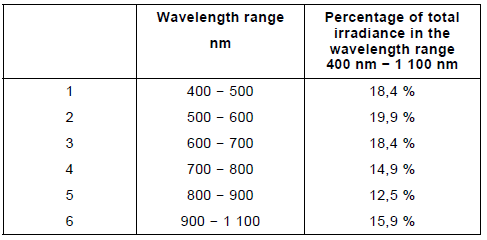
\includegraphics[width=75mm]{img/spectral.png}
\caption[Spektralle Strahlungsverteilung]{Spektralle Strahlungsverteilung nach IEC 60904-9}\label{rolle}
\end{figure}

\begin{figure}[htbp]
\centering
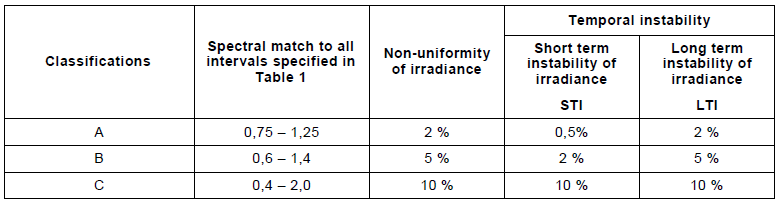
\includegraphics[width=75mm]{img/simclass.png}
\caption[Simulatorklassen]{Simulatorklassen}\label{Sim2}
\end{figure}



\section{Theorie Referenzzelle}
Referzelle, Temperaturabh"angikeit Messzelle, Kennlinine, Warum Kurzschlussstrom,...


\chapter{Entwicklungprozess}


\section{Hardwaredesign}
\subsection{Mecanum-Platform}
Das Mecanum-Rad ist ein Rad, das Fahrman"over in jede Richtung erlaubt, ohne dass das Fahrzeug mit einer mechnischen Lenkung ausgestattet ist. Bennnt ist es nach dem schwedischen Unternehmen Macanum AB in welchen dieses Rad 1971 entwickelt wurde. 
Erreicht wird die Wendigkeit der Fahrzeuge durch den Einsatz von Mecanum R"adern, die einzeln angetrieben werden. Diese R"ader bestehen aus einer Felge, auf der unter einem Winkel von 45 Grad lose, ballige Rollen so angebracht sind, dass sie "uber den Abrollumfang wieder einen exakten Kreis bilden.
Durch die Schr"aganordnung der Rollen entstehen beim Antreiben des Rades 2 Kraftkomponenten. Gegeneinander gerichtete Kr"afte der einzelnen R"ader werden "uber die Achsen und den Rahmen kompensiert. Die "ubrigen Kr"afte addieren sich zur resultierenden Fahrtrichtung. Auf diese Weise kann durch entsprechendes Ansteuern der einzelnen R"ader bez"uglich Drehrichtung und -geschwindigkeit jedes beliebige Fahrman"over erzeugt werden.
\begin{figure}[htbp]
\centering
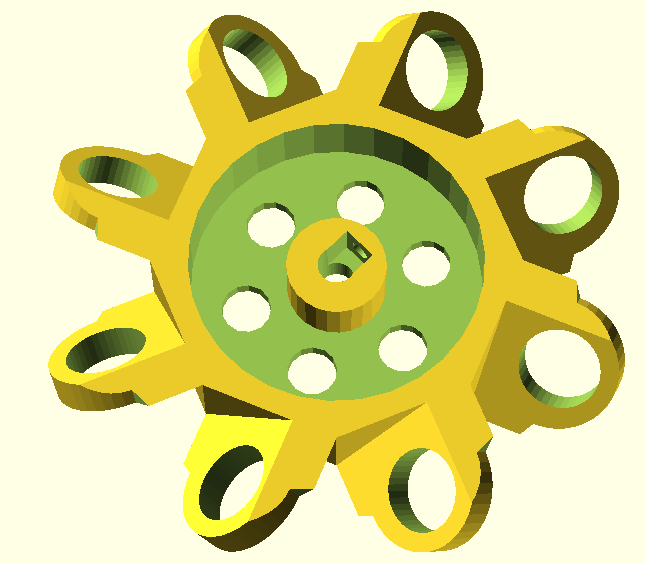
\includegraphics[width=75mm]{img/wheel.png}
\caption[Mecanum-Rad]{Mecanum-Rad}\label{rad}
\end{figure}

\begin{figure}[htbp]
\centering
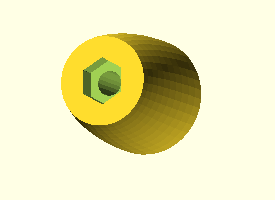
\includegraphics[width=75mm]{img/roller.png}
\caption[Rolle]{Rolle}\label{rolle}
\end{figure}

\begin{figure}[htbp]
\centering
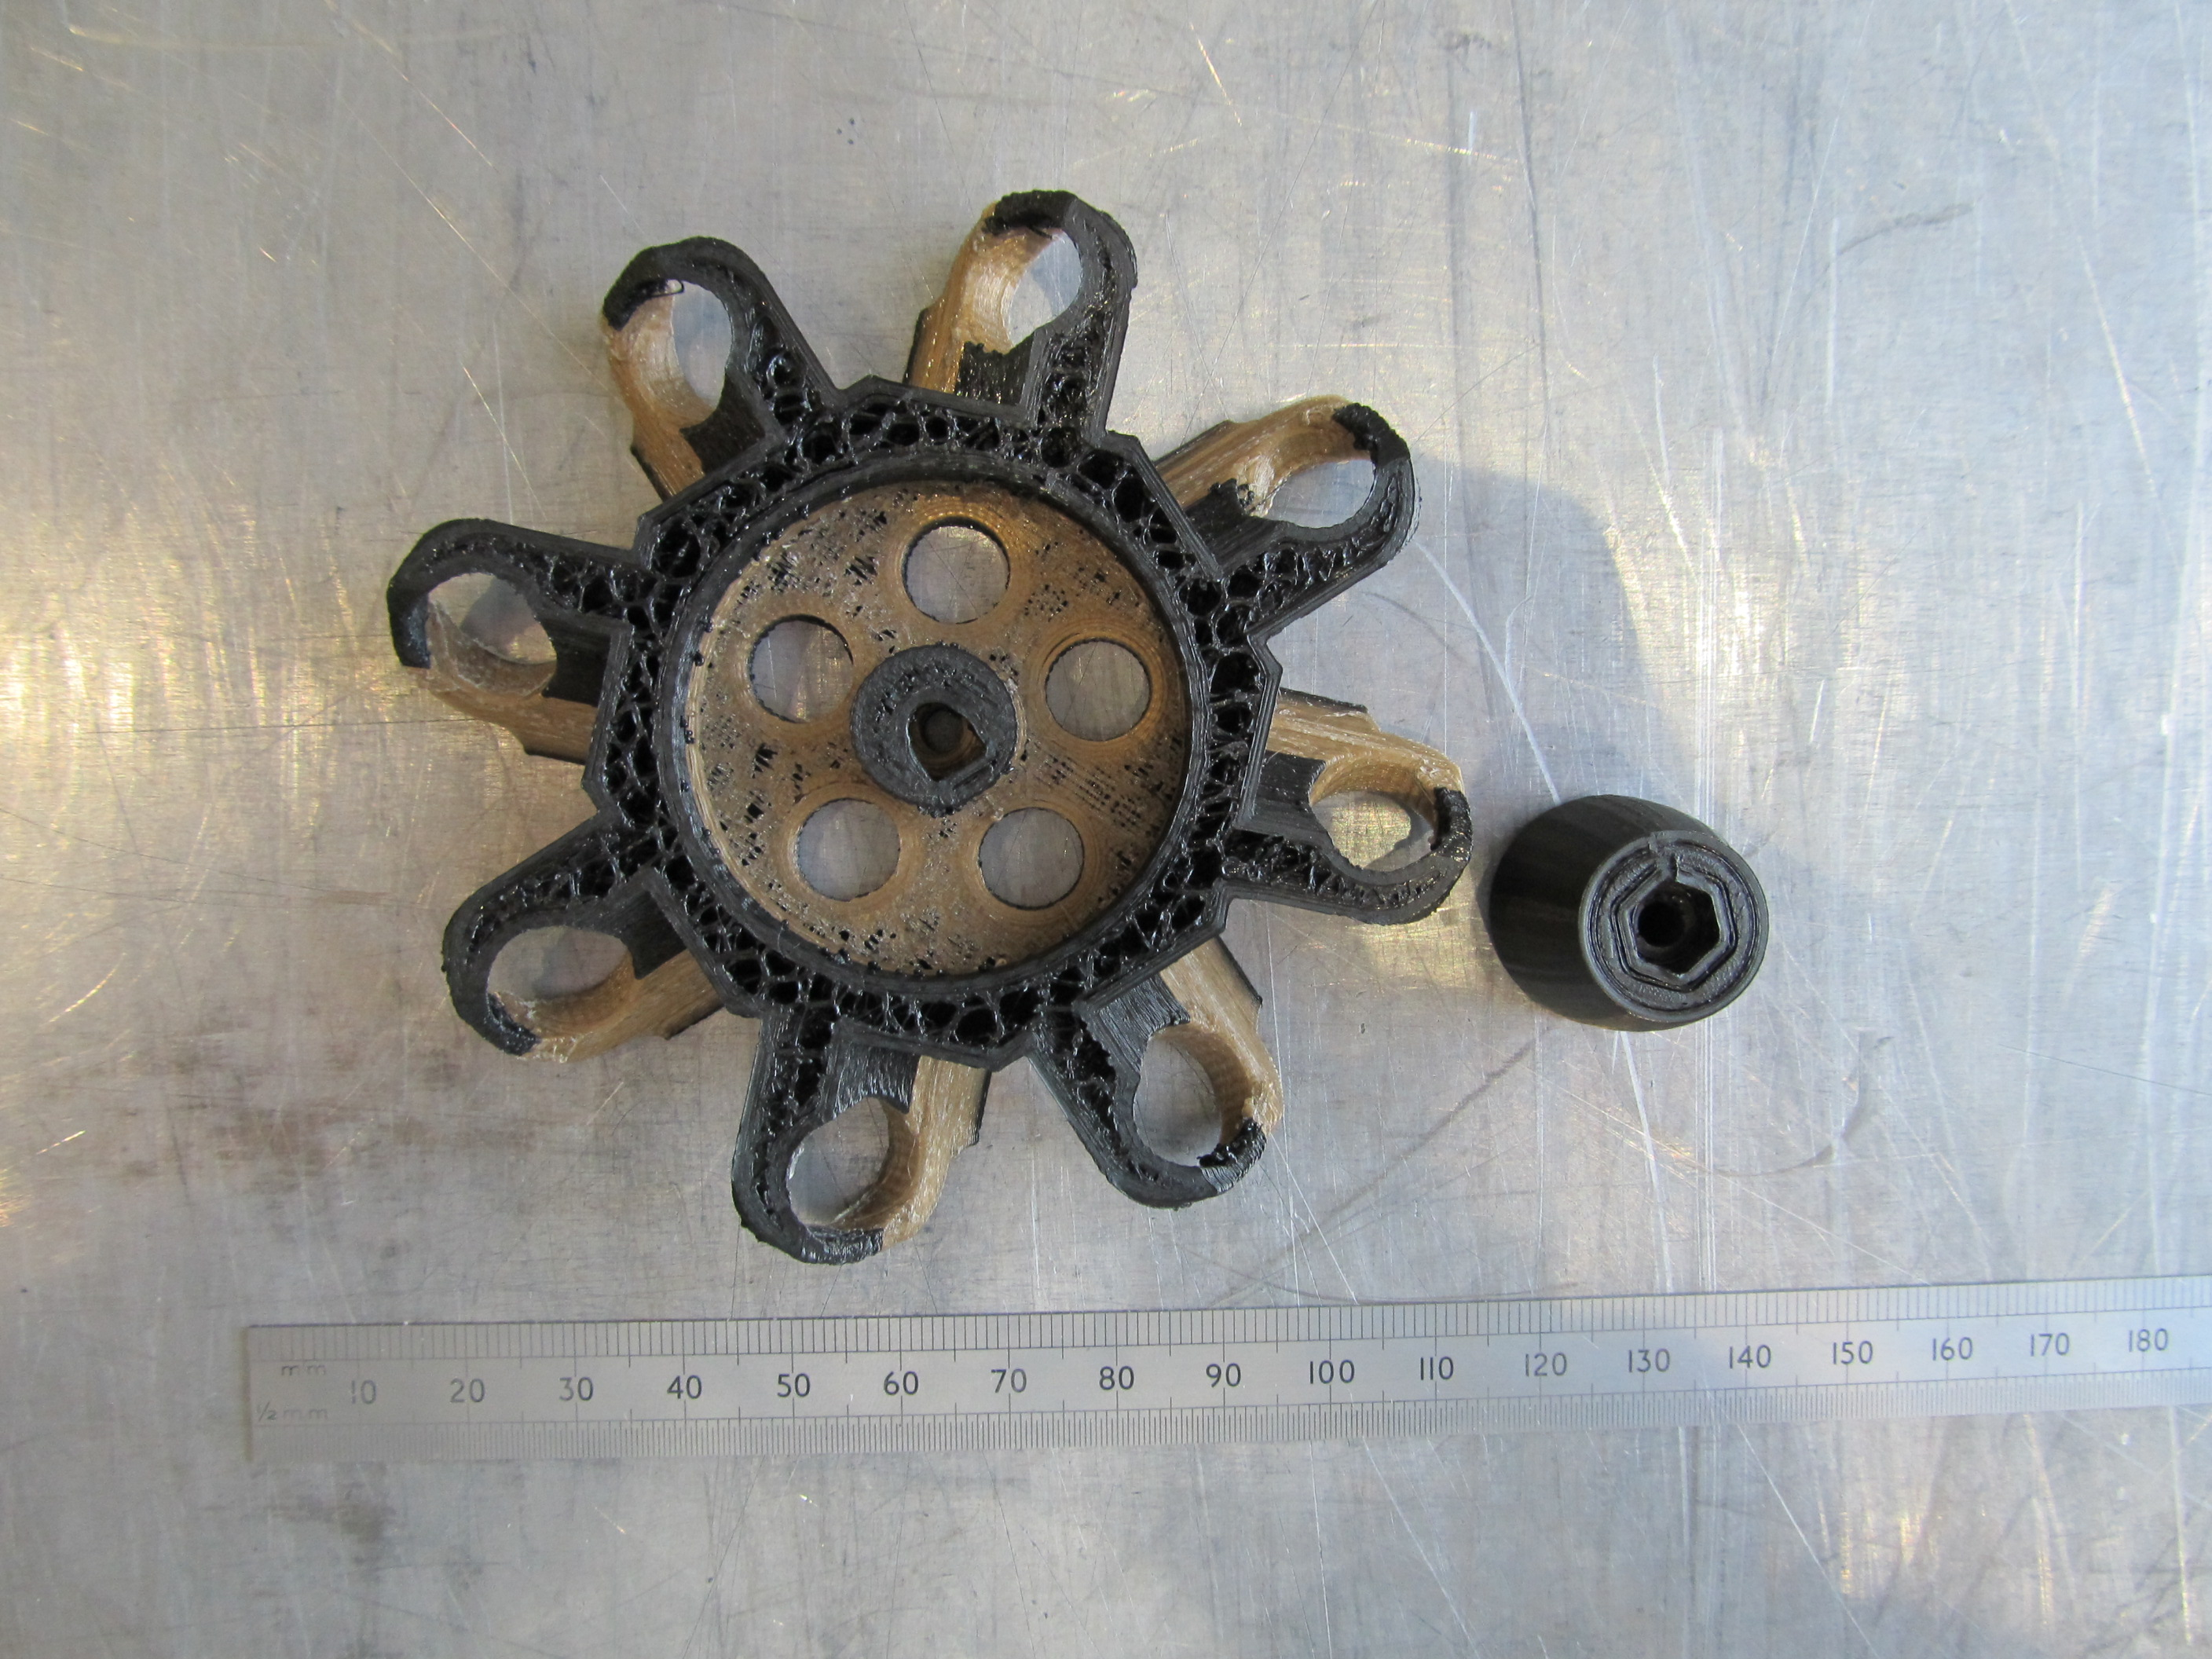
\includegraphics[width=75mm]{img/roller_wheel.jpg}
\caption[Foto eines gedruckten Rades]{Foto eines gedruckten Rades}\label{rollerad}
\end{figure}

\subsection{Chassis}
Die Chassis wurde aus Verbund-Holz gefertigt. Das Design dafür entstand mit QCAD. Die Einzelteile wurden mit einem Lasercutter aus einer großen Platte geschnitten. Dann verschraubt und teilweise geleimt. Der Oberteil des Chassis lässt sich von der Bodenplatte trennen.
Die Motoren sind verschraubt. Einzelne Räder und auch Rollen lassen sich bei Bedarf austauschen.
Das Chassis besteht aus 3 Teilen: \newline
- die Bodenplatte
\newline
- die Seitenwände
\newline
- das Dach mit der Aufnahme für die Messzelle
\newline

\begin{figure}[htbp]
\centering
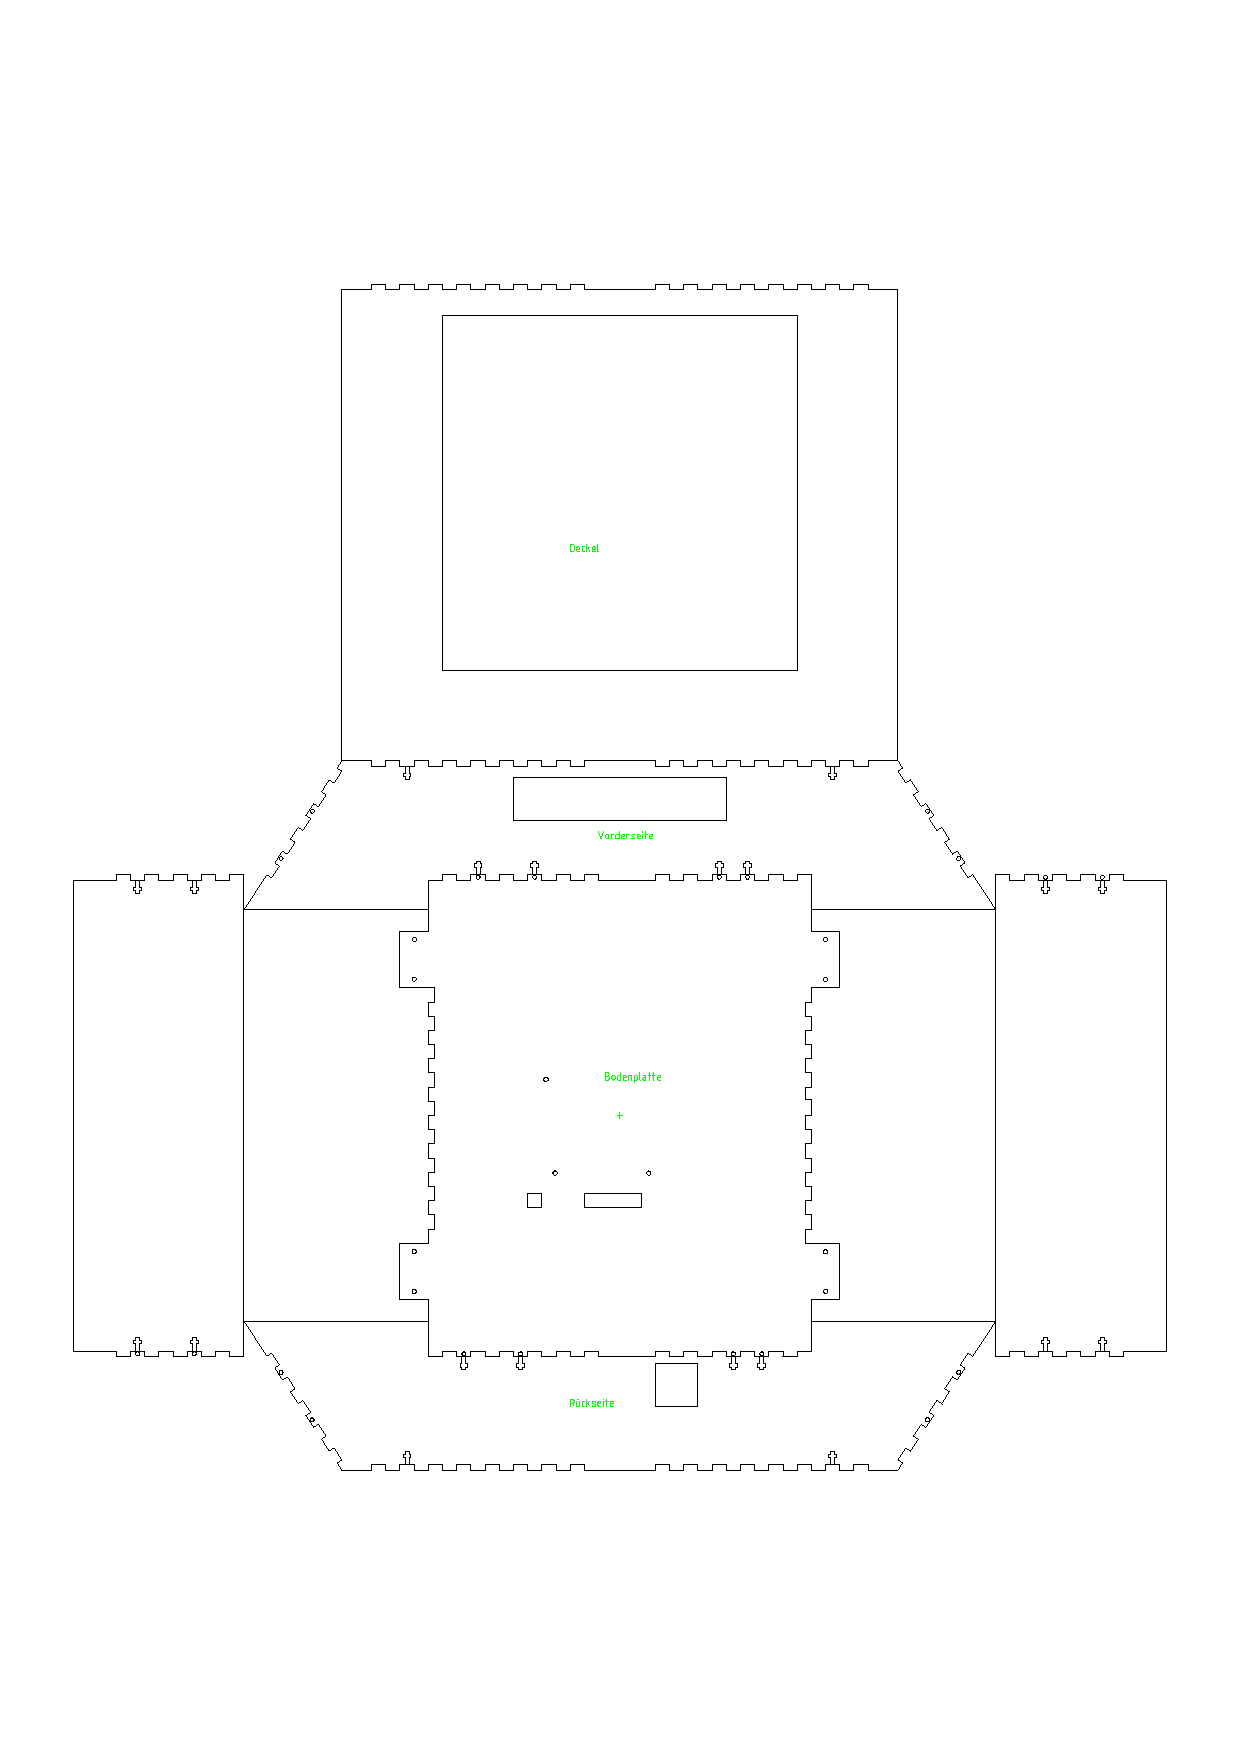
\includegraphics[width=125mm]{img/gehause.pdf}
\caption[Chassis]{Chassis}\label{chassis}
\end{figure}


\section{Steuerungselektronik}
\subsection{Motorensteuerung}
H-Br"ucken Treiber: NJM2670
The NJM2670 is a general-purpose 60V dual H-bridge
drive IC. It consists of a pair of H-bridges, a thermal shut
down circuit and its alarm output. The alarm output can
detect application problems and the system reliability will be
significantly improved if monitored by Micro Processor.
Therefore, it is suitable for two-phase stepper motor
application driven by microprocessor.
Motor: Getriebemotor RB 35, 1:200
Versorgungsspannung: 12V wurde auf 15,5 bis 16 erh"oht
Drehzahl: 30 Umdrehungen pro Minute im Leerlauf bei 12V Versorgung
Achsdurchmesser: 6mm 

\subsection{Optische Sensorik}
Der Roboter ist ein Linienfolge. Damit er einer Linie folgen kann, muss diese zuerst zuverl"assig erkannt werden. 
Als Sensor wurde ein CNY70 verwendet. Der CNY 70 ist ein Reflexionsensor. Der Sensor wird in einem fixen Abstand zu einer Ebene montiert. Eine LED sendet Licht mit 950nm aus, welches an der Ebene reflektiert wird. Damit können Unterschiede des Reflektionkoeffizienten, umgangssprachlich der Farbe, gemessen werden. Die Anordung 9 solcher Sensoren in einem 3 mal 3 Array kann sowohl vertikale als auch horizontale Linien erkennen, sowie Ecken.

\begin{figure}[htbp]
\centering
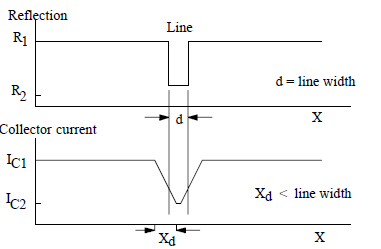
\includegraphics[width=75mm]{img/cny70.png}
\caption[...]{...}\label{cny1}
\end{figure}

\begin{figure}[htbp]
\centering
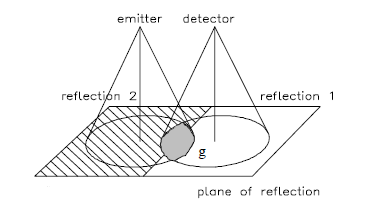
\includegraphics[width=75mm]{img/cny701.png}
\caption[...]{...}\label{cny1}
\end{figure}

\begin{figure}[htbp]
\centering
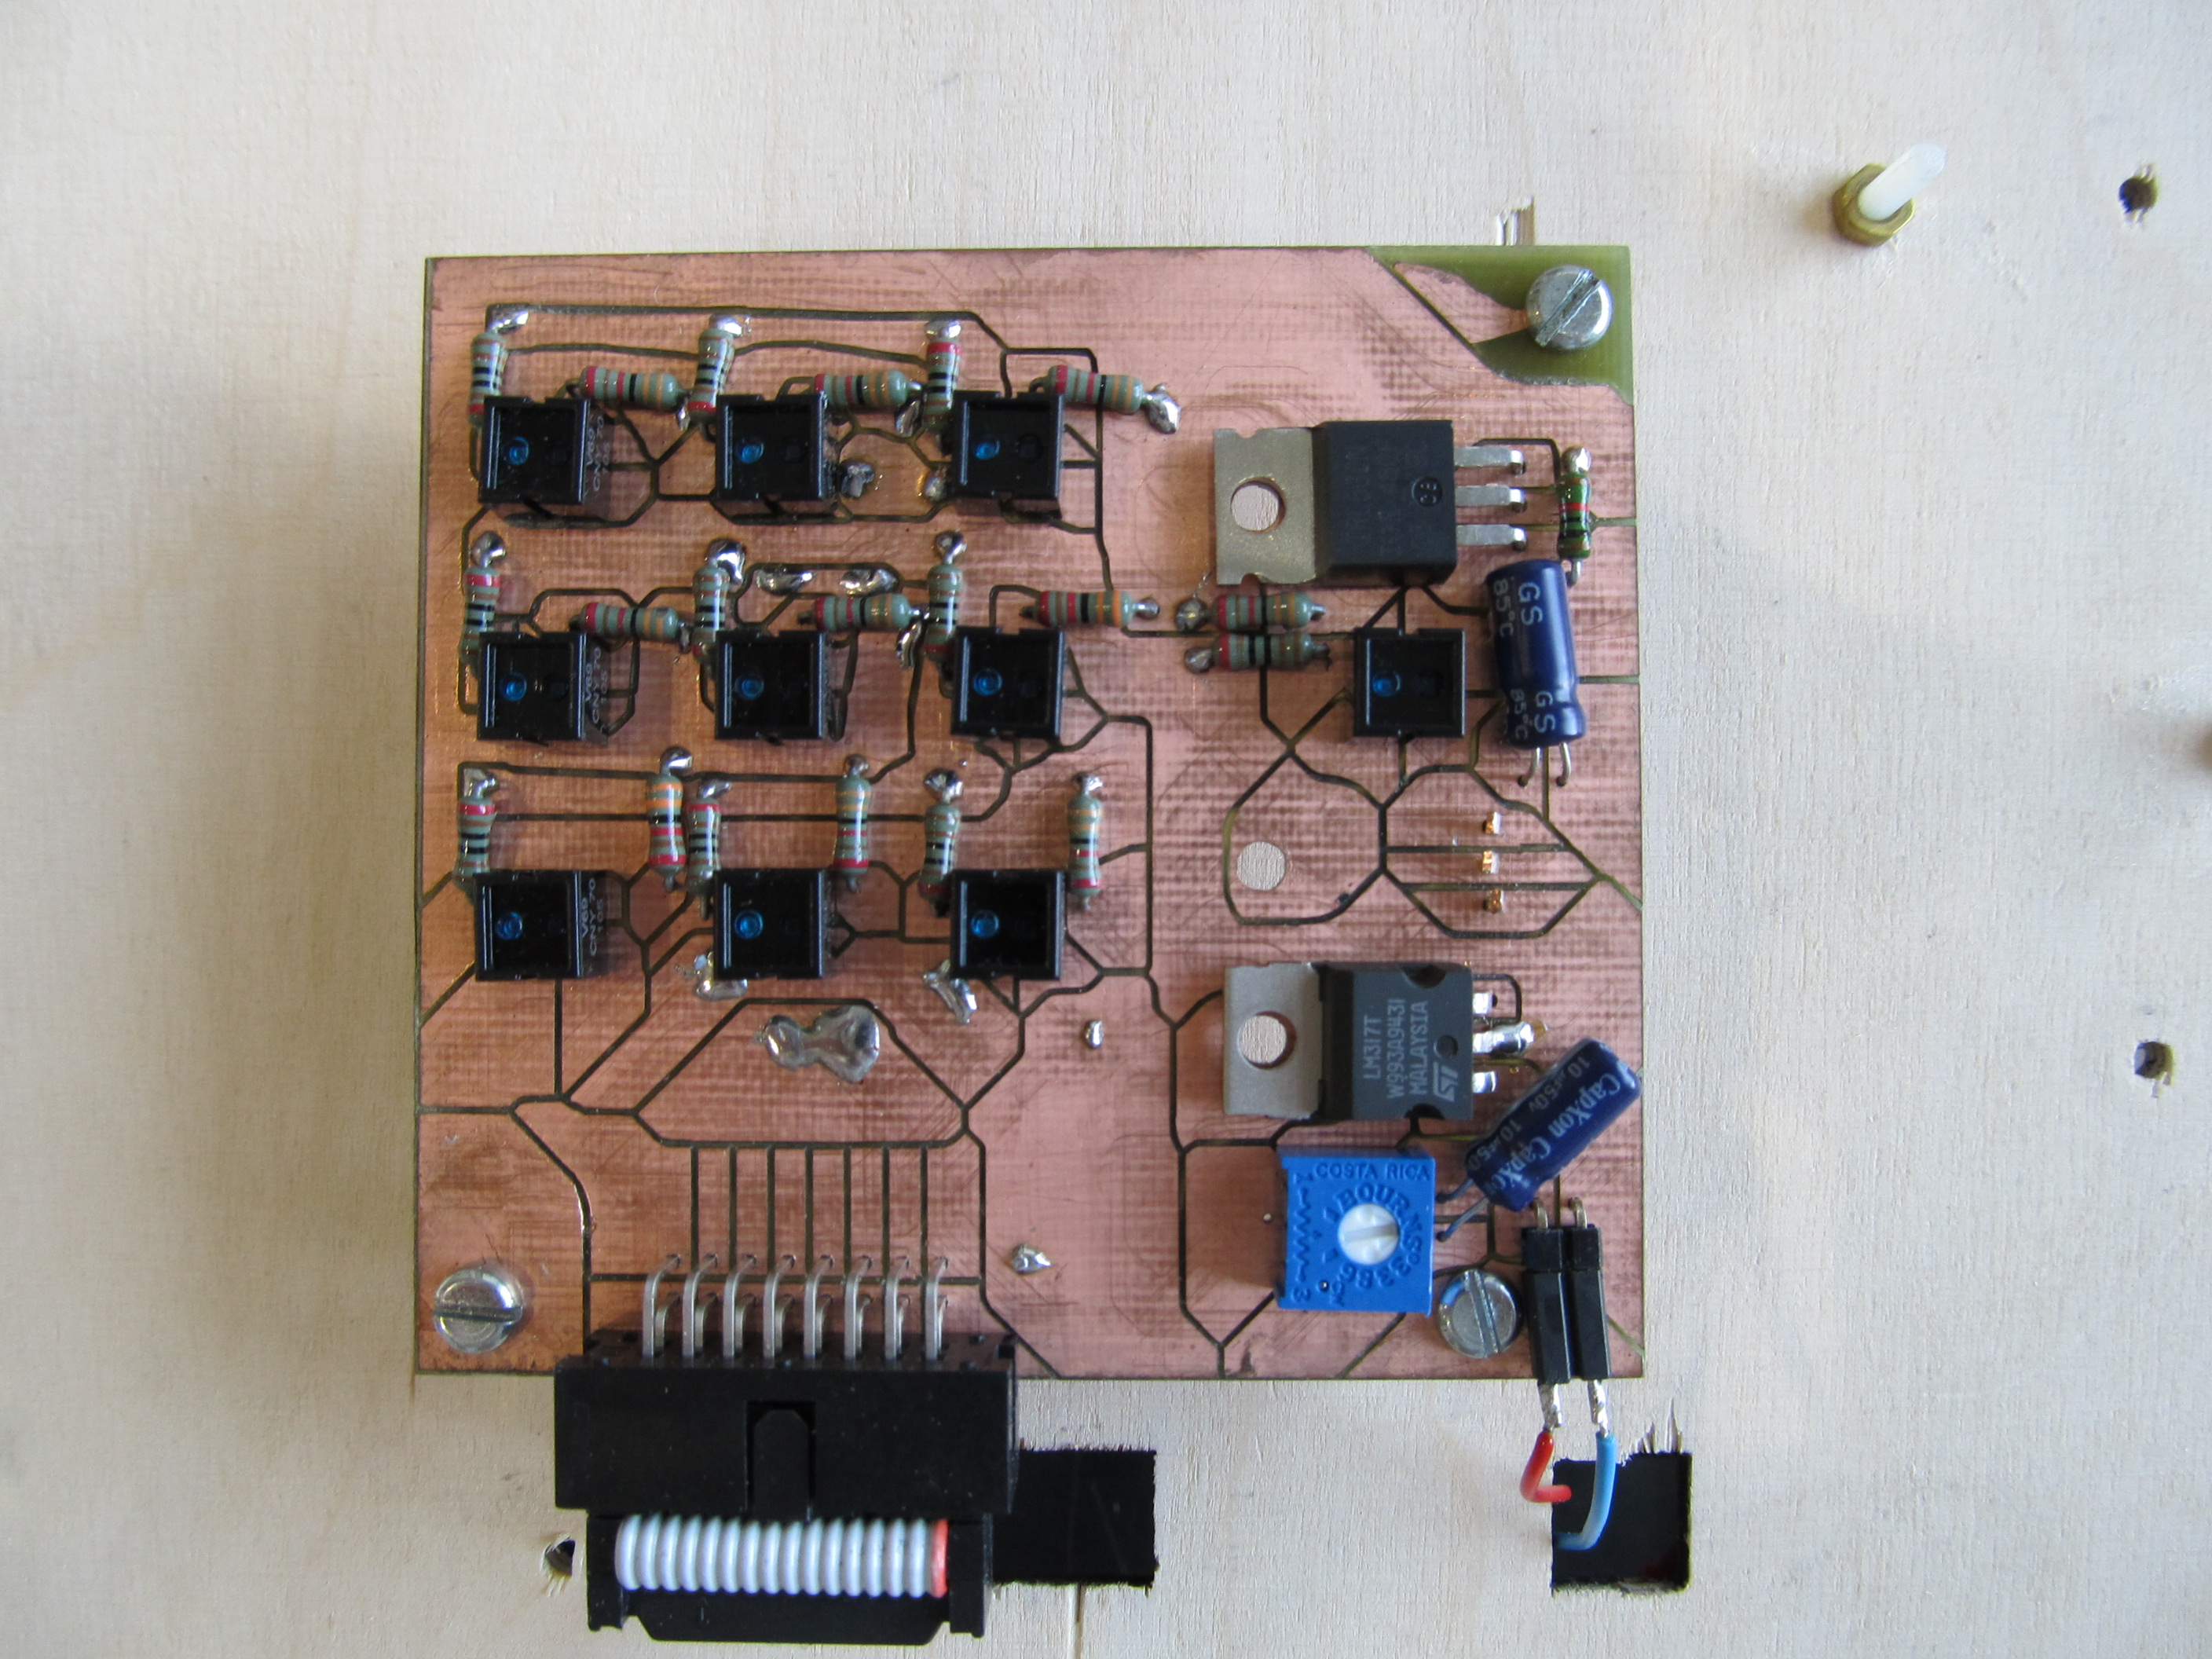
\includegraphics[width=125mm]{img/sensor_array.jpg}
\caption[Sensorarray]{Sensorarraf im Roboter eingebaut}\label{array3}
\end{figure}



\subsection{Spannungversorgung}
Aku-handling, "Uberwachung der Akkuspannung, Alarm und Abschaltung bei Unterspannung, 
Es wird empfohlen vor jeden Messzyklus den Akku zu laden. Ein voller Akku schafft ohne Probleme 10 Messfahrten. 
Bauteile: Akku, Ladeger"at (extern), bequemes und schnelles Laden des Akkus
Eine Schmelzsicherung ist direkt im Anschlusskabel des Akkus eingebaut. Der Akku schafft Ströme bis 200A, da er aus dem Modellbausektor kommt. Was für den Roboter völlig überdimensioniert ist. Der maximale Strom aller 4 Motoren und der restlichen Elektronik liegt bei einem Ampere. Die Motoren werden direkt mit der Akkuspannung versorgt. Da realistischerweise die Versorgungsspannung zwischen 16,4V (Akku voll) und 15,5V (nach vielen Fahrten) liegt, ist der Einfluss auf die Drehzahl der Motoren zu vernachl"assigen. 
Die 5 Volt Versorgung des Mikrocontrollers und der OPVs wurde mit einem RECOM R-785.0-1.0 DC-DC Konverter gelöst. Er ist pinkompatibel zu einem 7805, und bietet die Vorteile einer geringen Verlustleistung und einer sehr genauen Ausgangsspannung. 
Die Analog-Digitalwandlung des Arduino benötigt eine Referenzspannung. Das kann die Versorgungsspannung sein, was aber doch zu ungenau ist. 
The LT1021 is a precision reference with ultralow drift
and noise, extremely good long term stability and almost
total immunity to input voltage variations. The reference
output will both source and sink up to 10mA. Three
voltages are available: 5V, 7V and 10V. The 7V and 10V
units can be used as shunt regulators (two-terminal zeners)
with the same precision characteristics as the threeterminal
connection. Special care has been taken to minimize
thermal regulation effects and temperature
induced hysteresis.
\subsection{Mikrokontroller}
Arduino (was ist das), Shield, SD, Aref,

The Arduino Mega 2560 is a microcontroller board based on the ATmega2560 (datasheet). It has 54 digital input/output pins (of which 14 can be used as PWM outputs), 16 analog inputs, 4 UARTs (hardware serial ports), a 16 MHz crystal oscillator, a USB connection, a power jack, an ICSP header, and a reset button. It contains everything needed to support the microcontroller; simply connect it to a computer with a USB cable or power it with a AC-to-DC adapter or battery to get started. The Mega is compatible with most shields designed for the Arduino Duemilanove or Diecimila.

The Mega 2560 is an update to the Arduino Mega, which it replaces. 

\subsection{Temperatursensoren}
Messprinzip, Temperaturstabili"at

\section{Softwareentwicklung}
\subsection{Entwicklungsumgebung}
The microcontroller on the board is programmed using the Arduino programming language (based on Wiring) and the Arduino development environment (based on Processing). Arduino projects can be stand-alone or they can communicate with software running on a computer (e.g. Flash, Processing, MaxMSP). 


\subsection{Auswertung optische sensoren}
Differentielle Messung: Zwar liegen die optischen Sensoren auf der Unterseite des Roboters, aber da es im Sonnensimulator eine Einstrahlung von 1000 Watt pro Quadratmeter gibt, mit einem Anteil im spektralen Arbeitsbereich der optischen Sensoren CNY70, ist es notwendig den Einfluss des Streulichtes zu unterdrücken. Dazu wird einmal mit und einmal ohne eingeschalteter Infrarot-LED gemessen, dann der Dunkelwert vom Hellwert abgezogen.


Mathematik Auswertung,
Anhand der Werte der einzelnen optischen Sensoren wird die Lage der Linie relativ zum Mittelpunktes des Arrays bestimmt. 
Rohefassung: Die Methode der kleinsten Quadrate (engl.: method of least squares) ist das mathematische Standardverfahren zur Ausgleichungsrechnung. Dabei wird zu einer Datenpunktwolke eine Kurve gesucht, die möglichst nahe an den Datenpunkten verläuft. Die Daten können physikalische Messwerte, wirtschaftliche Größen oder Ähnliches repräsentieren, während die Kurve aus einer parameterabhängigen problemangepassten Familie von Funktionen stammt. Die Methode der kleinsten Quadrate besteht dann darin, die Kurvenparameter so zu bestimmen, dass die Summe der quadratischen Abweichungen der Kurve von den beobachteten Punkten minimiert wird. Die Abweichungen werden Residuen genannt.
\newline
Folge der Linie

Behandlung der Ecken

Haltepunkte
\subsection{Auswertung ADCs}
Mittelung, Rauschgr"oßen, 

\subsection{Programmablauf}
Das Programm startet im Modus Start, der Roboter steht, und wartet 60 Sekunden, eine Pufferzeit damit nach dem Einschalten des Roboters die Lade des Sonnensimulator hineingeschoben und die Klappe geschlossen werden kann.
Nach Ablauf dieser 60 Sekunden wechselt das Programm in den Modus Vorwärts. In diesem Modus fährt der Roboter in Vorwärtsrichtung. Abweichungen von der Idealspur werden erkannt und korrigiert. Wird mit dem Stopsensor eine Stopmarkierung erkannt, wechselt das Programm in den Messmodus.

\chapter{Kalibration}
\section{Temperatursensoren}
\section{Messzelle}

\begin{figure}[htbp]
\centering
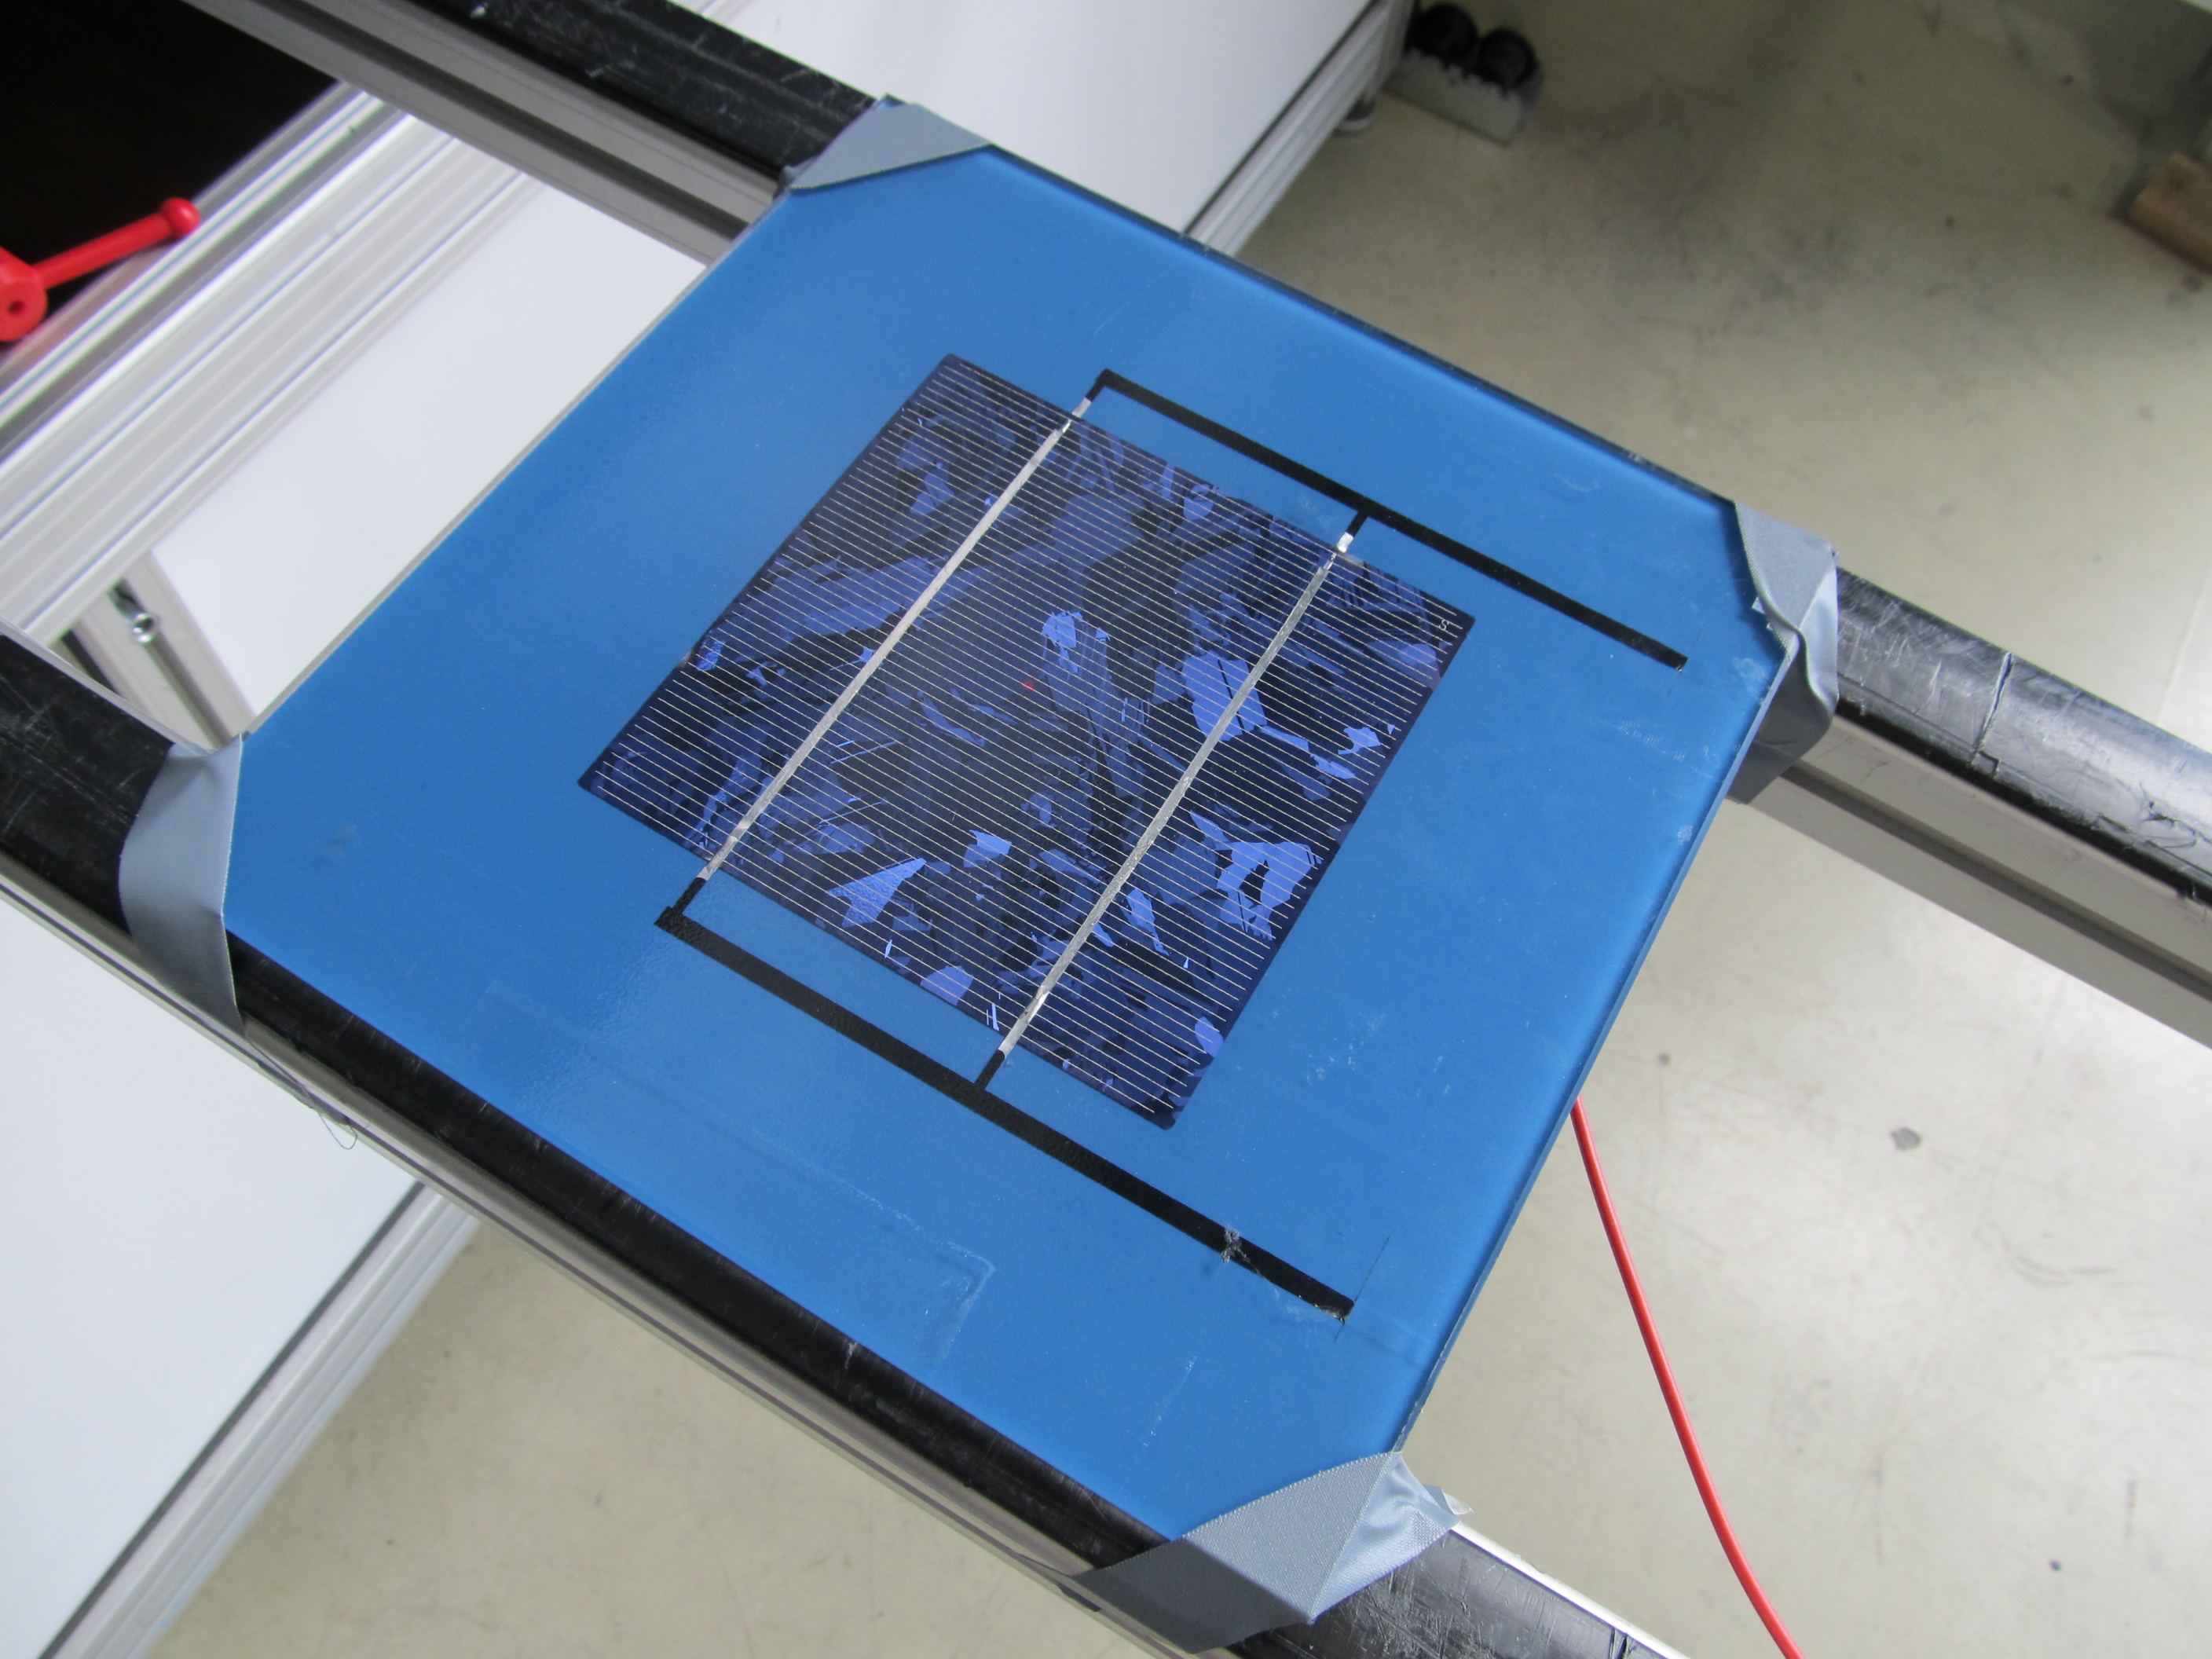
\includegraphics[width=75mm]{img/zelle.jpg}
\caption[Messzelle auf der Lade des Flashers]{Messzelle auf der Lade des Flashers}\label{zelleflasher}
\end{figure}

\begin{figure}[htbp]
\centering
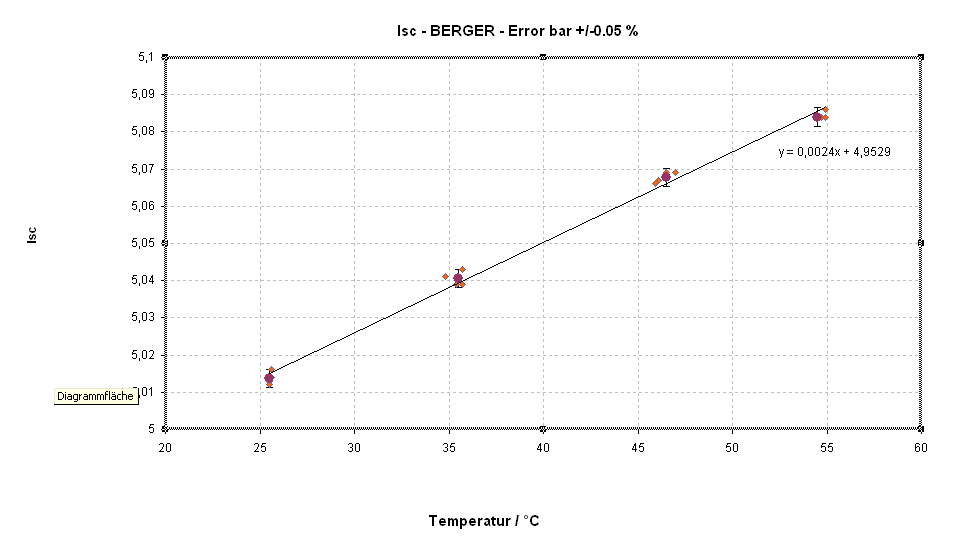
\includegraphics[width=125mm]{img/tempkoef.png}
\caption[Kurzschlusstrom "uber Temperatur]{Kurzschluusstrom "uber Temperatur}\label{tempkoef}
\end{figure}

\section{Strommessung}

\section{Thermische Stabilit"at}



\chapter{Messung}
\section{Messaufbau}
  \subsection{Platten}
  \subsection{Ablauf}
\section{Auswertung}


wie von sd  zu Bild,
gemessene Verteilungen,

Rohfassung: ADC Werte werden auf SD Karte gespeichert:
Zeit in ms, Isc, Temperatur des Moduls, Umgebungstemperatur, Messpunkt, Reihe, Spalte
Es sind 308 Messpunkte, 14 mal 22, es kann vorkommen, am Übergang von einer Platte zur anderen, dass ein Messpunkt ausgelassen wird. Das ist erkennbar wenn nicht 308 Messwerte im datalog-File sind. Um den Fehler leicht zu finden wurde Spalte und Reihe mit aufgezeichnet. Sind in einer Spalte nur 13 Messwerte, fehlt in dieser Spalte ein Wert. Anhand der mit aufgezeichneten Zeit kann der fehlende Messpunktes lokalisiert werden. Das geschiet nicht automatisch Der Messwert wird anhand der neben liegenden Werte geschätzt. Alternativ werden nur Messfahrten mit allen Punkten ausgewertet.

Auf der SD Karte sind alle Messwerte in einer Wurscht gespeichert. Für die visuelle Auswertung wird diese Datenwurst in ein zweidimensionales Array umgewandelt. 
Formel, Formel
Der ADC Wert des Kurschlussstromes wird in Ampere umgerechnet. Verwendet wird die in der Kallibrierung gewonnene Formel.

\section{Schlussfolgerung}

\begin{itemize}
\item Code: arduino, Matlab, fileformat
\end{itemize}


% Literaturverzeichnis
% Das Literaturverzeichnis kann auch nach einem allf"alligen Anhang positiioniert werden (siehe "`Leitfaden f"ur Bachelor- und Diplomarbeiten"', Version 2.0, Abschnitt 2.9).

% M"oglichkeit 1: Erzeugung des Literaturverzeichnisses mit BibTeX:
% Die Quellen sind in der Datei *.bib (hier Literatur.bib) einzugeben. Danach muss diese Vorlage einmal geTeXt werden, dann BibTeX angewendet werden und 
% anschliessend nochmals zweimal geTeXt werden.
% Im Text erfolgt die Zitierung mit dem Anker-Schl"usselwort, z.B. \cite{kop05}.
\bibliographystyle{IEEEtran}
\bibliography{Literatur}

% M"oglichkeit 2: Erzeugung eines Literaturverzeichnisses ohne BibTeX:
%\begin{thebibliography}{99}
%\bibitem[kop05]{kop05}
%H.~Kopka, {\em LaTeX, Band 1: Einf"uhrung}, Pearson Studium, M"unchen, 3.~Auflage, 2005.
%\bibitem[knu98]{knu98}
%F.~Mittelbach, M.~Goossens, J.~Braams, D.~Carlisle, and Ch. Rowley, {\em The LaTeX Companion}, 
%Addison-Wesley, 2nd edition, 2004.
%\end{thebibliography}

% Abbildungsverzeichnis
\listoffigures
\addcontentsline{toc}{chapter}{Abbildungsverzeichnis} % f"ugt den Eintrag "Abbildungsverzeichnis" im Inhaltsverzeichnis hinzu
\newpage

% Tabellenverzeichnis
\listoftables 
\addcontentsline{toc}{chapter}{Tabellenverzeichnis} % f"ugt den Eintrag "Tabellenverzeichnis" im Inhaltsverzeichnis hinzu
\newpage

% Abk"urzungsverzeichnis
% Bei Verwendung der Dokumentklasse "scrartcl" ist der Befehlt \addchap{Abk"urzungsverzeichnis} durch 
% \addsec{Abk"urzungsverzeichnis} zu ersetzen
\addchap{Abk"urzungsverzeichnis}
\hspace{-17mm}\begin{tabular}{>{\raggedleft}p{0.2\linewidth} p{0.75\linewidth} p{0.1\linewidth}}
www & World Wide Web \\
URL & Uniform Resource Locator
\end{tabular}


% Anh"ange
\begin{appendix}
\chapter{Sourcecode Arduino}

\begin{verbatim}
/*
Programm zum Steuern des Sonnensimulatormessroboters
 Version 1.0 
 */

#include <SD.h>

void vor(int sped);
void zuruck(int sped);
void left(int sped);
void right(int sped);
void tl(int sped);
void tr(int sped);
void ztl();
void ztr();
void vtl();
void vtr();
void halt(); 

// ADCs zum Auslesen der 3x3 Matrix
const int analogInPin0 = A9;  
const int analogInPin1 = A2;
const int analogInPin2 = A5;
const int analogInPin3 = A8;
const int analogInPin4 = A1;
const int analogInPin5 = A4;
const int analogInPin6 = A7;
const int analogInPin7 = A0;
const int analogInPin8 = A3;
const int analogInPin9 = A6;

// Ausgang zum Schalten der Infrarot-Leds
const int analogInPin10 = A10;

// ADC für Messwerte
const int analogInPin12 = A12;
const int analogInPin13 = A13;
const int analogInPin14 = A14;
const int analogInPin15 = A15;

// Digitalausg"ange zum Ansteuern der Motoren
int IN1M1 = 2;
int IN2M1 = 3;
int IN1M2 = 4;
int IN2M2 = 5;
int IN1M3 = 6;
int IN2M3 = 9;
int IN1M4 = 7;
int IN2M4 = 8;

// Sensorwerte der optischen Sensoren (beleuchtet)
int sensorValue0 = 0;        // value read from the pot
int sensorValue1 = 0;        // value read from the pot
int sensorValue2 = 0;        // value read from the pot
int sensorValue3 = 0;        // value read from the pot
int sensorValue4 = 0;        // value read from the pot
int sensorValue5 = 0;        // value read from the pot
int sensorValue6 = 0;        // value read from the pot
int sensorValue7 = 0;        // value read from the pot
int sensorValue8 = 0;        // value read from the pot
int sensorValue9 = 0;        // value read from the pot

// Sensorwerte der optischen Sensoren (unbeleuchtet)
int sensorValue0d = 0;        // value read from the pot
int sensorValue1d = 0;        // value read from the pot
int sensorValue2d = 0;        // value read from the pot
int sensorValue3d = 0;        // value read from the pot
int sensorValue4d = 0;        // value read from the pot
int sensorValue5d = 0;        // value read from the pot
int sensorValue6d = 0;        // value read from the pot
int sensorValue7d = 0;        // value read from the pot
int sensorValue8d = 0;        // value read from the pot
int sensorValue9d = 0;        // value read from the pot

// für Auswertung der opischen Sensoren
int A = 0;
int B = 0;
int C = 0;
int D = 0;
int E = 0;
int F = 0;
int G = 0;
int H = 0;
int I = 0;
int S = 0;

// Grenzwerte für hell (=white) und dunkel (=bleak)
int white = 400;
int white2 = 250;
int bleak = 100;
int bleak2 = 150;

// zur Berechnung der Lage der LInie
float x1,x2,x3,d,k;
float y1,y2,y3,d2,k2;

// einige Hilfsvariablen
char mode='s';
char richtung='v';
int _stop=0;
int vor_ein=0;
int zuruck_ein=0;

// für die Auswertung der Messwerte
long int  temp_modul = 0; 
long int temp_i=0;
long int _Isc = 0; 
long int time = 0; 

// zur Schreiben auf die SD Karte
const int chipSelect = 53;

// Z"ahlvariable für Messpunkt, Spalte und Reihe
int count = 0;
int count2 = 0;
int row = 1;

// zur Schreiben auf die SD Karte
String dataString = "";

// notwendig für die Kommunikation mit SD Karte
void setup() {
  pinMode(A10, OUTPUT);
  pinMode(53, OUTPUT);
  SD.begin(chipSelect);
}

// Definiert alle möglichen Bewegungen
void zuruck(int sped)  
{
  analogWrite(IN1M1,0);
  analogWrite(IN2M1,sped);   
  analogWrite(IN1M2,0);
  analogWrite(IN2M2,sped); 
  analogWrite(IN1M3,0);
  analogWrite(IN2M3,sped); 
  analogWrite(IN1M4,0);
  analogWrite(IN2M4,sped);
}  

void vor(int sped)  
{
  analogWrite(IN1M1,sped);
  analogWrite(IN2M1,0);   
  analogWrite(IN1M2,sped);
  analogWrite(IN2M2,0); 
  analogWrite(IN1M3,sped);
  analogWrite(IN2M3,0); 
  analogWrite(IN1M4,sped);
  analogWrite(IN2M4,0);
}

void left(int sped)  
{
  analogWrite(IN1M1,0);
  analogWrite(IN2M1,sped);   
  analogWrite(IN1M2,sped);
  analogWrite(IN2M2,0); 
  analogWrite(IN1M3,sped);
  analogWrite(IN2M3,0); 
  analogWrite(IN1M4,0);
  analogWrite(IN2M4,sped);
}

void right(int sped)  
{
  analogWrite(IN1M1,sped);
  analogWrite(IN2M1,0);   
  analogWrite(IN1M2,0);
  analogWrite(IN2M2,sped); 
  analogWrite(IN1M3,0);
  analogWrite(IN2M3,sped); 
  analogWrite(IN1M4,sped);
  analogWrite(IN2M4,0);
}

void tr(int sped)
{
  analogWrite(IN1M1,sped);
  analogWrite(IN2M1,0);   
  analogWrite(IN1M2,0);
  analogWrite(IN2M2,sped); 
  analogWrite(IN1M3,sped);
  analogWrite(IN2M3,0); 
  analogWrite(IN1M4,0);
  analogWrite(IN2M4,sped);
}

void tl(int sped)
{
  analogWrite(IN1M1,0);
  analogWrite(IN2M1,sped);   
  analogWrite(IN1M2,sped);
  analogWrite(IN2M2,0); 
  analogWrite(IN1M3,0);
  analogWrite(IN2M3,sped); 
  analogWrite(IN1M4,sped);
  analogWrite(IN2M4,0);
}

void vtr()
{   
  analogWrite(IN1M1,64);
  analogWrite(IN2M1,0);   
  analogWrite(IN1M2,0);
  analogWrite(IN2M2,64); 
  analogWrite(IN1M3,128);
  analogWrite(IN2M3,0); 
  analogWrite(IN1M4,128);
  analogWrite(IN2M4,0);
}

void vtl()
{   
  analogWrite(IN1M1,0);
  analogWrite(IN2M1,64);   
  analogWrite(IN1M2,64);
  analogWrite(IN2M2,0); 
  analogWrite(IN1M3,128);
  analogWrite(IN2M3,0); 
  analogWrite(IN1M4,128);
  analogWrite(IN2M4,0);
}

void ztr()  
{
  analogWrite(IN1M1,0);
  analogWrite(IN2M1,64);   
  analogWrite(IN1M2,0);
  analogWrite(IN2M2,64); 
  analogWrite(IN1M3,0);
  analogWrite(IN2M3,64); 
  analogWrite(IN1M4,64);
  analogWrite(IN2M4,0);
}  

void ztl()  
{
  analogWrite(IN1M1,0);
  analogWrite(IN2M1,64);   
  analogWrite(IN1M2,0);
  analogWrite(IN2M2,64); 
  analogWrite(IN1M3,64);
  analogWrite(IN2M3,0); 
  analogWrite(IN1M4,0);
  analogWrite(IN2M4,64);
}  

void halt()  
{
  analogWrite(IN1M1,0);
  analogWrite(IN2M1,0);   
  analogWrite(IN1M2,0);
  analogWrite(IN2M2,0); 
  analogWrite(IN1M3,0);
  analogWrite(IN2M3,0); 
  analogWrite(IN1M4,0);
  analogWrite(IN2M4,0);
}


// Hauptschleife
void loop() 
{

  // Werte ohne Beleuchtung:
  sensorValue0d = analogRead(analogInPin0);   
  sensorValue1d = analogRead(analogInPin1);  
  sensorValue2d = analogRead(analogInPin2);  
  sensorValue3d = analogRead(analogInPin3);  
  sensorValue4d = analogRead(analogInPin4);  
  sensorValue5d = analogRead(analogInPin5);  
  sensorValue6d = analogRead(analogInPin6);  
  sensorValue7d = analogRead(analogInPin7);  
  sensorValue8d = analogRead(analogInPin8);  
  sensorValue9d = analogRead(analogInPin9);  
  digitalWrite(A10, HIGH);  // LED ein
  delay(2); 
  // Werte mit Beleuchtung:
  sensorValue0 = analogRead(analogInPin0);   
  sensorValue1 = analogRead(analogInPin1);  
  sensorValue2 = analogRead(analogInPin2);  
  sensorValue3 = analogRead(analogInPin3);  
  sensorValue4 = analogRead(analogInPin4);  
  sensorValue5 = analogRead(analogInPin5);  
  sensorValue6 = analogRead(analogInPin6);  
  sensorValue7 = analogRead(analogInPin7);  
  sensorValue8 = analogRead(analogInPin8);  
  sensorValue9 = analogRead(analogInPin9);  
  digitalWrite(A10, LOW);

  A = sensorValue1 - sensorValue1d;
  B = sensorValue2 - sensorValue2d;
  C = sensorValue3 - sensorValue3d;
  D = sensorValue4 - sensorValue4d;
  E = sensorValue5 - sensorValue5d;
  F = sensorValue6 - sensorValue6d;
  G = sensorValue7 - sensorValue7d;
  H = sensorValue8 - sensorValue8d;
  I = sensorValue9 - sensorValue9d;

  S = sensorValue0 - sensorValue0d;

  // zum Erkennen der Linie bei vor- oder zurückfahren 
  x1 = ((C-A)/float(2*A-4*B+2*C));
  x2 = ((F-D)/float(2*D-4*E+2*F));
  x3 = ((I-G)/float(2*G-4*H+2*I));

  d = (x1 + x2 + x3)/3.; // ~ Abstand von der Ideallinie
  k = (x1-x3)/2.;  // Steigung = Verdrehung

  // zum Erkennen der Linie bei links- oder rechtsfahren
  y1 = ((G-A)/float(2*A-4*D+2*G));
  y2 = ((H-B)/float(2*B-4*E+2*H));
  y3 = ((I-C)/float(2*C-4*F+2*I));

  d2 = (y1+y2+y3)/3.;
  k2 = (y3-y1)/2.;

  if( S < bleak2) _stop=0;

  halt();

  if(E>bleak2)
  {

    switch(mode)
    {
    case 's':     // Start
      { 
        halt();
        delay(60000);  // 1 Minuten warten
        mode='v';
      }
      break;

      // Messmode
    case 'e':   // Ende
      {
        halt();
      }
      break;

    case 'm':   // Messen
      { 
        count = count + 1;  // Anzahl der Haltepunkte
        count2 = count2 + 1; 
        dataString = "";
        _stop=1;
        halt();

        delay(250);   // damit die Str"ome der Fahrmotoren keinen Einfluss auf die AD-Wandlung haben

        _Isc = 0;
        temp_modul = 0;
        temp_i = 0;

        // Mittelung über jeweils 500 Messwerte
        for(int i = 0; i < 500 ; i++)
        {
          _Isc = _Isc + analogRead(analogInPin13);  
          temp_modul = temp_modul + analogRead(analogInPin12); 
          temp_i =  temp_i + analogRead(analogInPin15); 
        }
        _Isc = int(_Isc/500.0);
        temp_modul = int(temp_modul/500.0);
        temp_i = int(temp_i/500.0);
        time = millis();

        // Schreiben aud SD-Karte
        dataString += String(time);
        dataString += "\t"; 
        dataString += String(_Isc); 
        dataString += "\t"; 
        dataString += String(temp_modul); 
        dataString += "\t"; 
        dataString += String(temp_i); 
        dataString += "\t"; 
        dataString += String(count); 
        dataString += "\t"; 
        dataString += String(count2); 
        dataString += "\t"; 
        dataString += String(row); 

        // Schreibe aud SD Card
        File dataFile = SD.open("datalog.txt", FILE_WRITE);
        if (dataFile) {
          dataFile.println(dataString);
          dataFile.close();
        }

        // zurück in den Bewegungsmode
        if(richtung=='v') mode='v';
        if(richtung=='z') mode='z';

      }
      break;

    case 'v':   // Vorwärtsfahren
      { 

        richtung='v';

        if(d>0.02)  vtr();
        else 
        {  
          if(d>-0.02)  vor(128);
          else 
            vtl();
        }

        //if((C<bleak)&&(A<bleak))
        if(A<bleak2)
        {
          if(k>0.01) tr(64);
          else
          {
            if(k<-0.01) tl(64);
          }

          if(d>0.025) right(64);
          else
          {
            if(d<-0.025) left(64);
          }
        }   
        if((A>white)&&(B>white)) mode='a'; 

        if((_stop==0)&&(S>white2)) mode='m';   


      }
      break;

    case 'z': // Rückwärtsfahren
      { 

        richtung='z';

        if(d>0.02)  ztr();
        else 
        {  
          if(d>-0.02)  zuruck(128);
          else  ztl();
        }

        //if((G<bleak)&&(I<bleak))
        if(G<bleak2)
        {
          if(k>0.01) tr(64);
          else
          {
            if(k<-0.01) tl(64);
          }

          if(d>0.025) right(64);
          else
          {
            if(d<-0.025) left(64);
          }
        }
        if((G>white)&&(H>white)) mode='c';

        if((_stop==0)&&(S>white2)) mode='m';  

        if((I<bleak)&&(H<bleak)&&(G<bleak)) mode='e';

      }
      break; 

    case 'r':     //nach rechts
      {
        richtung='r';
        count2 = 0;

        right(128);
        if(D>white2)
        {
          if(d2>0.04) vor_ein=1;
          if(d2<0.02) vor_ein=0;
          if(d2<-0.04) zuruck_ein=1;
          if(d2>-0.02) zuruck_ein=0;

          if(vor_ein==1) vor(64);
          if(zuruck_ein==1) zuruck(64);

          if((vor_ein==0)&&(zuruck_ein==0))
          {
            if(k2>0.02) tr(64);
            else
            {
              if(k2<-0.02) tl(64);
            }
          }
        }

        if((D<bleak)&&(G<bleak)&&(A<bleak)) 
        { 
          mode='b';
        }

      } 
      break;

    case 'l':    // auch nach rechts 
      {
        richtung=='l';
        count2 = 0;

        right(128);
        //if((C<bleak)&&(I<bleak))
        if(D>white2)
        {
          if(d2>0.04) vor_ein=1;
          if(d2<0.02) vor_ein=0;
          if(d2<-0.04) zuruck_ein=1;
          if(d2>-0.02) zuruck_ein=0;

          if(vor_ein==1) vor(64);
          if(zuruck_ein==1) zuruck(64);

          if((vor_ein==0)&&(zuruck_ein==0))
          {
            if(k2>0.02) tr(64);
            else
            {
              if(k2<-0.02) tl(64);
            }
          }
        }

        if((D<bleak)&&(G<bleak)&&(A<bleak))
        { 
          mode='d';
        }

      } 
      break;

    case 'a':  // Um die Ecke fahren
      {
        if((A>bleak2)&&(B>bleak2)) vor(64);
        else 
        { 
          right(64);
          delay(700);
          halt();
          row = row +1 ;

          mode='r';

        }
      } 
      break; 

    case 'b':  // Um die Ecke fahren
      {

        zuruck(64);
        delay(850);
        halt();
        delay(500);

        mode='x';

      } 
      break; 

    case 'x':
      {
        if(d>0.025) right(64);

        if(d<-0.025) left(64);

        if((d<0.1)&&(d>-0.1)) mode='y';
      }
      break;

    case 'y':
      {
        if(k>0.01) tr(32);

        if(k<-0.01) tl(32);

        if((k<0.04)&&(k>-0.04)) mode='z';
      }
      break;

    case 'c':  // Um die Ecke fahren
      {
        if((H>bleak2)&&(G>bleak2 )) zuruck(64);
        else 
        { 
          right(64);
          delay(700);
          halt();
          row = row +1 ;

          mode='l';
        }
      } 
      break; 

    case 'd':  // Um die Ecke fahren
      {

        vor(64);
        delay(850);
        halt();
        delay(500);
        mode='q';

      } 
      break; 

    case 'q':
      {
        if(d>0.025) right(64);

        if(d<-0.025) left(64);

        if((d<0.1)&&(d>-0.1))       mode='p';
      }
      break;


    case 'p':
      {
        if(k>0.01) tr(32);

        if(k<-0.01) tl(32);

        if((k<0.04)&&(k>-0.04)) mode='v'; 

      }
      break;
    } 
  }   


  else 
  {  
    if((richtung=='v')||(richtung=='z'))
    {
      if((A>bleak2)||(D>bleak2)||(G>bleak2)||(C>bleak2)||(F>bleak2)||(I>bleak2))
      {
        if((A+D+G)>(C+F+I)) right(128);
        else left(128);
      }
      else halt();
    }


    if((richtung=='r')||(richtung=='l'))
    {
      if((A>bleak2)||(B>bleak2)||(C>bleak2)||(G>bleak2)||(H>bleak2)||(I>bleak2))
      {
        if((A+B+C)>(G+H+I)) vor(64);
        else zuruck(64);
      }
      else halt();
    }
  }

  delay(5); 

}
\end{verbatim}

\chapter{Sourcecode Auswertung}



\begin{verbatim}

% Graphische Auswertung der Robotermesswerte

close all;
clc;
clear all;

% "Offnen der Datei, welche eine Messfahrt mit genau 308 Messwerten
% enthalten muss
fid = fopen('data1.txt', 'r');
a = fscanf(fid, '%g %g', [7 308])     
a = a';
fclose(fid)

j=1; k=1; l=1;

% Umwandeln der 1 dimensionalen Modultemperatur ADC-Werte in eine Matrix:
for(i=0:307)
    if(mod(i,28)>13) k = 28- mod(i,28);
    else k = mod(i,14)+1;
    end
    Tm(k,l)=a(i+1,3);
    if(mod(i+1,14)==0) l=l+1;
    end
end

% Umrechnung der ADC-Werte in Temeratur:
Rm = (Tm +4038.9)/40.107;  % ADC --> Widerstand
TTm = (Rm-100.03)/0.3879;  % Widerstand --> Temperatur

j=1; k=1; l=1;

% Umwandeln der 1 dimensionalen Innentemperatur ADC-Werte in eine Matrix:
for(i=0:307)
    if(mod(i,28)>13) k = 28- mod(i,28);
    else k = mod(i,14)+1;
    end
    Ti(k,l)=a(i+1,4);
    if(mod(i+1,14)==0) l=l+1;
    end
end

% Umrechnung der ADC-Werte in Temeratur:
Ri = (Ti +4023.6)/40.027;  % ADC --> Widerstand
TTi = (Ri-100.03)/0.3879;  % Widerstand --> Temperatur

j=1; k=1; l=1;

% Umwandeln der 1 dimensionalen Kurzschlusstrom ADC-Werte in eine Matrix:
for(i=0:307)
    if(mod(i,28)>13) k = 28- mod(i,28);
    else k = mod(i,14)+1;
    end
    I(k,l)=a(i+1,2);
    if(mod(i+1,14)==0) l=l+1;
    end
end

% Umrechnung der ADC-Werte in Ampere:

A = (I +4.5766)/119.2;   % ADC --> Ampere
A = A - (TTm-25)*0.004;  % Temperaturkorrektur



[XI,YI] = meshgrid(1:.125:22, 1:.125:14);

Ai = interp2(A,XI,YI,'cubic'); % Interpolation

A_max = max(max(Ai));
A_min = min(min(Ai));

Normiert = Ai / A_max * 1.1;

w = (A_max - A_min)/(A_max + A_min) * 100  % maximale Abweichung in Protzent

% Graphische Darstellung des Stromes
figure;
surf(XI,YI,Ai);   % in Ampere


% Graphische Darstellung des normierten Stromes
zlevs2 = 0.9:0.01:1.1;
figure;
[C,h] = contourf(XI,YI,Normiert,zlevs2);
set(h,'ShowText','on','TextStep',get(h,'LevelStep')*2)
colorbar;

% Graphische Darstellung der Modultemperatur
figure;
surf(TTm); 

% Graphische Darstellung der Umgebungstemperatur
figure;
surf(TTi);

\end{verbatim} 

\end{appendix}


\end{document}
